\documentclass{beamer}

\usepackage{comment}
\usepackage{color}
\usepackage{listings}
\usepackage{verbatim}
\usepackage{multicol}
\usepackage{booktabs}
\usepackage{textpos}
\usepackage{graphicx}
\usepackage{graphics}
\definecolor{green}{RGB}{0,128,0}

\newcommand\gehcomment[1]{{{\color{orange} #1}}}
\newcommand\add[1]{{{\color{blue} #1}}}
\newcommand\remove[1]{\sout{{\color{red} #1}}}
\newcommand\codecomment[1]{{{\color{green} #1}}}
\newcommand\redcomment[1]{{{\color{red} #1}}}
\newcommand\bluecomment[1]{{{\color{blue} #1}}}
\newcommand\greencomment[1]{{{\color{green} #1}}}
\newcommand\magentacomment[1]{{{\color{magenta} #1}}}

\begin{document}
\title{Injection Well\ldots}
\author{Michael Nole}
\date{\today}

%\frame{\titlepage}

%-----------------------------------------------------------------------------
\section{Description of Injection Well Scenario}

\subsection{Injection Well Conceptual Model}

\frame{\frametitle{Description of Injection Well Scenario}

The ``Injection Well Scenario'' simulates 2D migration of CO2 injected into a heterogeneous reservoir using the fully coupled well model, using Webb extensions, and considering gas trapping hysteresis in \bluecomment{SCO2 MODE}.

This demonstration covers the following:

\begin{itemize}
  \small
  \item Set up a 2D heterogeneous model with a fully coupled hydrostatic well in SCO2 mode.
  \item Run the simulation.
  \item Visualize results in Paraview.
\end{itemize}
}

%-----------------------------------------------------------------------------
\section{Description of Input Deck}

%-----------------------------------------------------------------------------
\subsection{DESCRIPTION}

\begin{frame}[fragile,allowframebreaks]\frametitle{DESCRIPTION}

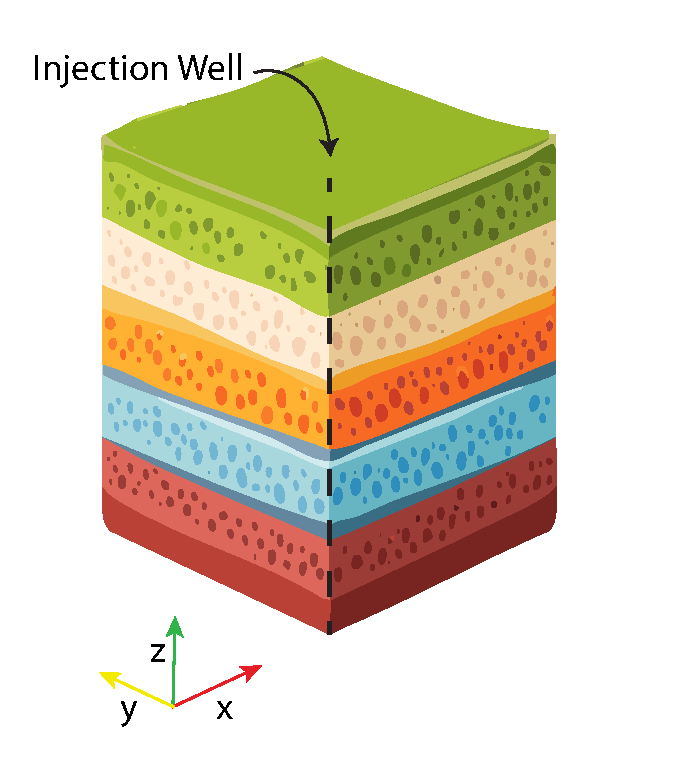
\includegraphics[height=3in]{injection-well-fig.pdf}

\newpage
\begin{itemize}
  \item 1. Initialize to hydrostatic conditions, isothermal temperature.
  \item 2. Well model occupies the left edge of the domain, is cased (unperforated) through the caprock and is perforated through the reservoir units.
  \item 3. Inject CO2 at 1 MMT/yr for 2 years.
\end{itemize}

\end{frame}

%-----------------------------------------------------------------------------
\subsection{SIMULATION\_INJECTION\_WELL}

\begin{frame}[fragile,allowframebreaks]\frametitle{SIMULATION: Injection Well}

\begin{itemize}
\item Specify SCO2 flow mode
\item Add checkpointing
\end{itemize}


\begin{semiverbatim}
SIMULATION
  SIMULATION_TYPE SUBSURFACE
  PROCESS_MODELS
    SUBSURFACE_FLOW flow
      MODE SCO2
      OPTIONS
        ISOTHERMAL_TEMPERATURE 25.d0
        NO_STATE_TRANSITION_OUTPUT
      /
    /
\newpage
    WELL_MODEL well1
      OPTIONS
        FLOW_COUPLING FULLY_IMPLICIT
        TYPE HYDROSTATIC
      END
    END
  /
END

SUBSURFACE
...

\end{semiverbatim}

\end{frame}

%-----------------------------------------------------------------------------
\subsection{NUMERICAL METHODS}
\begin{frame}[fragile]\frametitle{NUMERICAL METHODS}

\begin{itemize}
  \item Numerical Methods within subsurface block
  \item Newton Solver and Linear Solver sub-blocks
\end{itemize}

\begin{semiverbatim}
NUMERICAL_METHODS flow
  NEWTON_SOLVER
    USE_INFINITY_NORM_CONVERGENCE
    NUMERICAL_JACOBIAN
    MINIMUM_NEWTON_ITERATIONS 2
    CENTRAL_DIFFERENCE_JACOBIAN
    CONVERGE_ON_WELL_RESIDUAL
    RESIDUAL_SCALED_INF_TOL 1.d-4
  END

  TIMESTEPPER FLOW
    TIMESTEP_MAXIMUM_GROWTH_FACTOR 1.25
  END
END

\end{semiverbatim}
\end{frame}

%-----------------------------------------------------------------------------
\subsection{WELL MODEL}
\begin{frame}[fragile,allowframebreaks]\frametitle{WELL MODEL}

\begin{itemize}
  \item Set up well grid and well properties
\end{itemize}

\begin{semiverbatim}
WELLBORE_MODEL well1
  WELL_GRID
    WELL_TRAJECTORY
      SURFACE_ORIGIN 2.5d0 5.d0 -965.d0
      SEGMENT_DXYZ CASED 0.d0 0.d0 -15.04d0
      SEGMENT_DXYZ UNCASED 0.d0 0.d0 -176.9838d0
    /
  /

\newpage
  WELL
    DIAMETER 0.3d0
    FRICTION_COEFFICIENT 1.d0
    WELL_INDEX_MODEL PEACEMAN_3D
    SKIN_FACTOR 0.d0
  /

  USE_WELL_COUPLER

END
\newpage
WELL_MODEL_OUTPUT
  WELL_LIQ_PRESSURE
  WELL_GAS_PRESSURE
  WELL_LIQ_Q
  WELL_GAS_Q
/

\end{semiverbatim}
\end{frame}
%-----------------------------------------------------------------------------
\subsection{GRID}
\begin{frame}[fragile,containsverbatim]\frametitle{GRID}

\begin{itemize}
  \item Cartesian grid, converted to an unstructured implicit mesh.
\end{itemize}

\begin{semiverbatim}
GRID
  # nx=20 x ny=1 x nz=25
  TYPE UNSTRUCTURED mesh.ugi
END
\end{semiverbatim}

\end{frame}
%-----------------------------------------------------------------------------
\subsection{FLUID\_PROPERTIES}
\begin{frame}[fragile,containsverbatim,allowframebreaks]\frametitle{Fluid Properties}

\begin{itemize}
  \item Define properties of water and gas
  \begin{itemize}
    \item Diffusion coefficients
    \item Equations of state
  \end{itemize}
\end{itemize}

\begin{semiverbatim}
FLUID_PROPERTY
  PHASE LIQUID
  DIFFUSION_COEFFICIENT 2.d-9
END

FLUID_PROPERTY
  PHASE GAS
  DIFFUSION_COEFFICIENT 2.d-5
END

\newpage

EOS WATER
  DENSITY IF97
  ENTHALPY IF97
  STEAM_DENSITY IF97
  STEAM_ENTHALPY IF97
  SATURATION_PRESSURE IF97
END

EOS GAS
  CO2_DATABASE ../../../../../database/co2_sw.dat
  HENRYS_CONSTANT DEFAULT
END

\end{semiverbatim}

\end{frame}
%-----------------------------------------------------------------------------
\subsection{MATERIAL\_PROPERTY}

\begin{frame}[fragile,containsverbatim,allowframebreaks]\frametitle{MATERIAL\_PROPERTY}

\begin{semiverbatim}
MATERIAL_PROPERTY caprock
  ID 1
  CHARACTERISTIC_CURVES caprock
  POROSITY 0.07
  TORTUOSITY 1.d0
  ROCK_DENSITY 2650.d0
  THERMAL_CONDUCTIVITY_DRY 2.d0
  THERMAL_CONDUCTIVITY_WET 2.18d0
  HEAT_CAPACITY 1000 J/kg-C
  PERMEABILITY
    PERM_ISO 5.6254628e-20
  /
  SOIL_COMPRESSIBILITY_FUNCTION LINEAR
  POROSITY_COMPRESSIBILITY 1.07618e-13
  SOIL_REFERENCE_PRESSURE 1.2d7
END \newpage
MATERIAL_PROPERTY Reservoir24
  ID 2
  CHARACTERISTIC_CURVES Reservoir24
  POROSITY 0.13
  TORTUOSITY 1.d0
  ROCK_DENSITY 2650.d0
  THERMAL_CONDUCTIVITY_DRY 2.d0
  THERMAL_CONDUCTIVITY_WET 2.18d0
  HEAT_CAPACITY 1000 J/kg-C
  PERMEABILITY
    PERM_ISO 1.9146312e-14
  /
  SOIL_COMPRESSIBILITY_FUNCTION LINEAR
  POROSITY_COMPRESSIBILITY 5.3809001e-14
  SOIL_REFERENCE_PRESSURE 1.2d7
END
\end{semiverbatim}
\newpage
\begin{itemize}
  \item +23 more reservoir units
\end{itemize}

\end{frame}

%-----------------------------------------------------------------------------
\subsection{CHARACTERISTIC\_CURVES}

\begin{frame}[fragile,containsverbatim, allowframebreaks]\frametitle{CHARACTERISTIC\_CURVES}

\begin{itemize}
\item Set Brooks-Corey parameters
\end{itemize}

\begin{semiverbatim}
CHARACTERISTIC_CURVES caprock
  SATURATION_FUNCTION BROOKS_COREY
    \greencomment{MAX_TRAPPED_GAS_SAT 0.2}
    \greencomment{UNSATURATED_EXTENSION}
    ALPHA 0.00001020408
    LAMBDA 0.8311
    LIQUID_RESIDUAL_SATURATION 0.0597
    MAX_CAPILLARY_PRESSURE 1.d9
  / 
\newpage
\begin{itemize}
\item BURDINE-BC relative permeability
\end{itemize}
  PERMEABILITY_FUNCTION BURDINE_BC_LIQ
    PHASE LIQUID
    LAMBDA 0.8311
    LIQUID_RESIDUAL_SATURATION 0.0597
  /
  PERMEABILITY_FUNCTION BURDINE_BC_GAS
    PHASE GAS
    LAMBDA 0.8311
    LIQUID_RESIDUAL_SATURATION 0.0597
    GAS_RESIDUAL_SATURATION 0.0597
  /
END
\end{semiverbatim}

\newpage

\begin{semiverbatim}
CHARACTERISTIC_CURVES Reservoir24
  SATURATION_FUNCTION BROOKS_COREY
    \greencomment{MAX_TRAPPED_GAS_SAT 0.2}
    \greencomment{UNSATURATED_EXTENSION}
    ALPHA 0.00008503401
    LAMBDA 0.8311
    LIQUID_RESIDUAL_SATURATION 0.0597
    MAX_CAPILLARY_PRESSURE 1.d9
  /
\newpage
  PERMEABILITY_FUNCTION BURDINE_BC_LIQ
    PHASE LIQUID
    LAMBDA 0.8311
    LIQUID_RESIDUAL_SATURATION 0.0597
  /
  PERMEABILITY_FUNCTION BURDINE_BC_GAS
    PHASE GAS
    LAMBDA 0.8311
    LIQUID_RESIDUAL_SATURATION 0.0597
    GAS_RESIDUAL_SATURATION 0.0597
  /
END
\end{semiverbatim}

\newpage
\begin{itemize}
  \item +23 more reservoir units
\end{itemize}

\end{frame}

%-----------------------------------------------------------------------------
\subsection{OUTPUT}

\begin{frame}[fragile,allowframebreaks]\frametitle{OUTPUT}

\begin{semiverbatim}

OUTPUT
  SNAPSHOT_FILE
    TIMES y 1.d-2 1.d-1 1.d0
    PERIODIC TIME 1.d0 y
    FORMAT HDF5
  /
  UNFILTER_NON_STATE_VARIABLES
\newpage  VARIABLES
   TEMPERATURE
   LIQUID_PRESSURE
   GAS_PRESSURE
   LIQUID_SATURATION
   GAS_SATURATION
   PRECIPITATE_SATURATION
   TRAPPED_GAS_SATURATION
   LIQUID_MASS_FRACTIONS
   GAS_MASS_FRACTIONS
   LIQUID_DENSITY
   GAS_DENSITY
   PERMEABILITY
   LIQUID_RELATIVE_PERMEABILITY
   GAS_RELATIVE_PERMEABILITY
  /
END
\end{semiverbatim}

\end{frame}

%-----------------------------------------------------------------------------
\subsection{TIME}

\begin{frame}[fragile]\frametitle{TIME}

\begin{itemize}
\item Run simulation to 10 y
\end{itemize}

\begin{semiverbatim}

TIME
  FINAL_TIME 1.d1 y
  INITIAL_TIMESTEP_SIZE 1.d-5 y
  MAXIMUM_TIMESTEP_SIZE 5.d-1 y
END

\end{semiverbatim}

\end{frame}

%-----------------------------------------------------------------------------
\subsection{REGION}

\begin{frame}[fragile,containsverbatim,allowframebreaks]\frametitle{REGION}

\begin{itemize}
  \item Delineate regions in the 2D domain for:
  \begin{itemize}
    \item east face
    \item caprock
    \item reservoir units
  \end{itemize}
\end{itemize}

\begin{semiverbatim}
REGION all
  COORDINATES
    0.d0    0.d0 -1157.024d0
    3048.d0 1.d3 -965.d0
  /
END
\newpage

REGION edge
  FACE EAST
  FILE mesh_ugi_east.ss
END

\newpage
REGION caprock
  COORDINATES
    0.d0    0.d0 -980.24
    3048.d0 1.d3 -965.9112d0
  /
END

REGION Reservoir24
  COORDINATES
    0.d0    0.d0 -983.288
    3048.d0 1.d3 -980.24
  /
END
\end{semiverbatim}
\begin{itemize}
  \item + 23 reservoir units
\end{itemize}
\end{frame}

%-----------------------------------------------------------------------------
\subsection{FLOW\_CONDITION}

\begin{frame}[fragile,allowframebreaks]\frametitle{FLOW\_CONDITION}

\newpage
\begin{semiverbatim}
FLOW_CONDITION initial
  TYPE
    LIQUID_PRESSURE HYDROSTATIC
    CO2_MASS_FRACTION DIRICHLET
    SALT_MASS_FRACTION DIRICHLET
  /
  DATUM 0.d0 0.d0 -1040.892d0
  LIQUID_PRESSURE 1.234333924d7
  CO2_MASS_FRACTION 0.d0
  SALT_MASS_FRACTION 4.75d-2
END

\newpage
FLOW_CONDITION injection
  SYNC_TIMESTEP_WITH_UPDATE
  TYPE
    RATE MASS_RATE
  /
  # 1.0 MMT/yr for 2 years
  RATE LIST
    TIME_UNITS y
    DATA_UNITS kg/y kg/y kg/y
    0.d0 0.d0 1.d9 0.d0
    2.d0 0.d0 0.d0 0.d0
  /
END
\end{semiverbatim}

\end{frame}

%-----------------------------------------------------------------------------
\subsection{INITIAL\_CONDITION}

\begin{frame}[fragile]\frametitle{INITIAL\_CONDITION}

\begin{semiverbatim}
INITIAL_CONDITION all
  FLOW_CONDITION initial
  REGION all
END

\end{semiverbatim}

\end{frame}

%-----------------------------------------------------------------------------
\subsection{BOUNDARY\_CONDITION}

\begin{frame}[fragile]\frametitle{BOUNDARY\_CONDITION}

\begin{itemize}
\item Couple the \greencomment{injection} flow condition with well model \greencomment{well1} and \greencomment{east} boundary condition with its corresponding region.
\end{itemize}

\begin{semiverbatim}
WELL_COUPLER injection
  FLOW_CONDITION injection
  WELL well1
END

BOUNDARY_CONDITION edge
  FLOW_CONDITION initial
  REGION edge
END
\end{semiverbatim}

\end{frame}

%-----------------------------------------------------------------------------

\subsection{STRATA}

\begin{frame}[fragile]\frametitle{STRATA}

\begin{semiverbatim}

STRATA
  REGION caprock
  MATERIAL caprock
END

STRATA
  REGION Reservoir24
  MATERIAL Reservoir24
END

...

END_SUBSURFACE
\end{semiverbatim}

\end{frame}

%-----------------------------------------------------------------------------
\subsection{buoyant-flow.in}

\begin{frame}[fragile]\frametitle{Running PFLOTRAN}

\begin{semiverbatim}

> cd \$PFLOTRAN_DIR
> cd shortcourse/exercises/co2/sco2/injection-well
> ./build_grid.sh
> pflotran -input_prefix injection-well
> paraview \&

\end{semiverbatim}

\end{frame}
\end{document}
